\chapter{Results}

The goal of this chapter is to analyse data generated by the algorithm presented in \cref{chp:generating-geodesics}.

\section{Growth Functions}

This section will provide a comparison of the geodesic and regular growth functions of the Fabrykowski-Gupta group.
The corresponding raw data of this section is provided in \cref{tab:strict-growths}.
Firstly, the regular and geodesic growth functions, $\gamma(n)$ and $\Gamma(n)$, are plotted in \cref{fig:normalGrowth}.

\begin{figure}[!h]
	\centering
	
	\begin{subfigure}{0.48\linewidth}
		\centering
		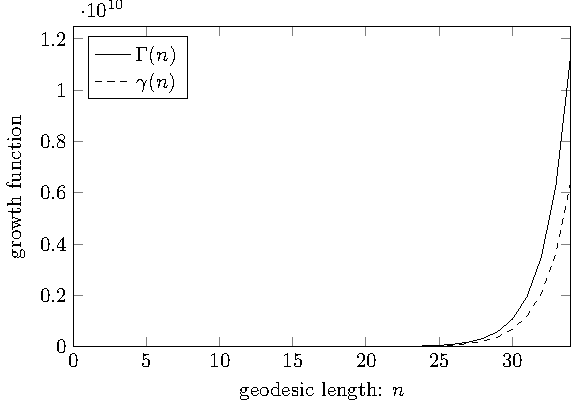
\includegraphics[width=\linewidth]
			{figures/results/normalGrowth/usual/normalGrowth}
		\caption{linear scale}
		\label{fig:normalGrowth:linear}
	\end{subfigure}
	\hfill
	\begin{subfigure}{0.48\linewidth}
		\centering
		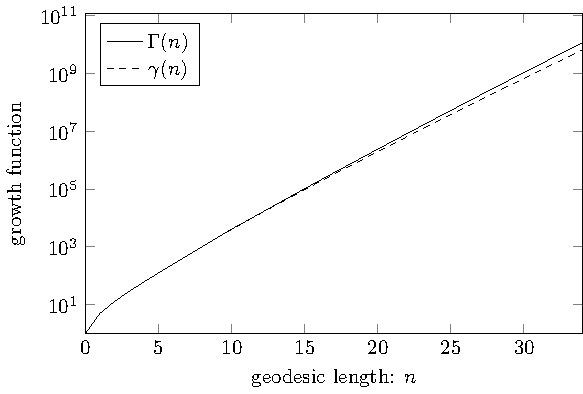
\includegraphics[width=\linewidth]
			{figures/results/normalGrowth/log/normalGrowthLog}
		\caption{logarithmic scale}
		\label{fig:normalGrowth:log}
	\end{subfigure}
	
	\caption{Comparison of the regular and geodesic growth functions}
	\label{fig:normalGrowth}
\end{figure}

Not much can be determined from \cref{fig:normalGrowth} as provided above.
Thus, to compare these two growth functions, the ratio $\Gamma(n)/\gamma(n)$ will instead be considered.
The ratio  $\Gamma(n)/\gamma(n)$ is of particular relevance as it can be shown that if this function is subexponential, then $\Gamma(n)$ would be of intermediate growth as would be desired.
An argument for this is given as follows.

We know  that $\Gamma(n)$ is superpolynomial since $\gamma \preccurlyeq \Gamma$ (see \cref{prop:growth-function-bounds}) and $\gamma(n)$ being superpolynomial \cite{OnGrowth}.
Also, it is known from \cite{OnGrowth} that $\gamma(n)$ is subexponential.
Hence, if $\Gamma(n)/\gamma(n)$ is subexponential, it would follow that the growth rate $\omega(\Gamma)$ could be computed as follows
\[
  \omega(\Gamma)
  =
  \lim_{n \to \infty}
  \frac{\log \Gamma(n)}{n}
  =
  \lim_{n \to \infty}
  \left(
  \frac{\log \gamma(n)}{n}
  +
  \frac{\log (\Gamma(n)/\gamma(n))}{n}
  \right)
  =
  \omega(\gamma)
  +
  \omega(\Gamma/\gamma)
\]
Then, since $\omega(\gamma) = 0$ and $\omega(\Gamma/\gamma) = 0$ by the definition of subexponential functions (see \cref{def:subexponential}), it follows that $\omega(\Gamma) = 0$; and thus $\Gamma(n)$ is subexponential.
Therefore, if $\Gamma(n)/\gamma(n)$ is subexponential, then it would follow that $\Gamma(n)$ is of intermediate growth.

Notice also that if $\Gamma(n)/\gamma(n)$ is exponential, then $\Gamma(n)$ would also be exponential.
This is clear as $\Gamma(n)/\gamma(n) \leq \Gamma(n)$ and thus $\Gamma/\gamma \preccurlyeq \Gamma$.
Thus, it can be seen that, if $\log(\Gamma(n)/\gamma(n))$ is linear, it would follow that $\Gamma(n)$ is exponential.
Hence, the function $\log(\Gamma(n)/\gamma(n))$ will also be considered.

Thus, consider the plots provided in \cref{fig:normalGrowthRatio}.

\begin{figure}[!h]
	\centering
	
	\begin{subfigure}{0.48\linewidth}
		\centering
		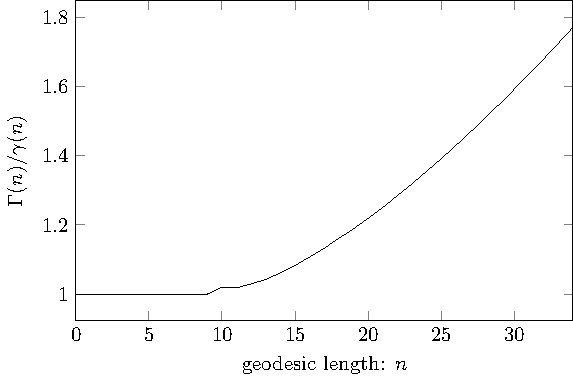
\includegraphics[width=\linewidth]
			{figures/results/normalGrowth/usual/normalGrowthRatio}
		\caption{Check for subexponential growth}
		\label{fig:normalGrowthRatio:linear}
	\end{subfigure}
	\hfill
	\begin{subfigure}{0.48\linewidth}
		\centering
		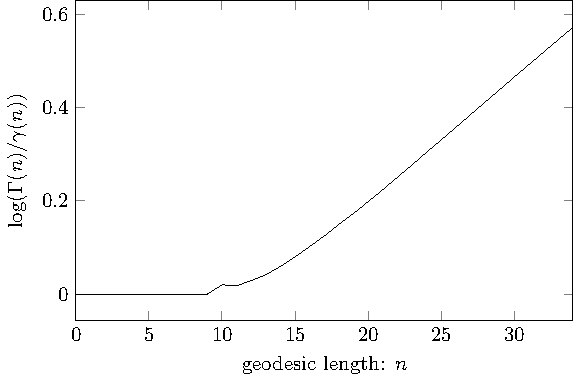
\includegraphics[width=\linewidth]
			{figures/results/normalGrowth/log/normalGrowthRatioLog}
		\caption{Check for exponential growth}
		\label{fig:normalGrowthRatio:log}
	\end{subfigure}
	
	\caption{Plots of $\Gamma(n)/\gamma(n)$ and $\log(\Gamma(n)/\gamma(n))$}
	\label{fig:normalGrowthRatio}
\end{figure}

The first derivatives (computed by the central difference) of these ratios are given in \cref{fig:normalGrowthRatioD1}.

\begin{figure}[!h]
	\centering
	
	\begin{subfigure}{0.48\linewidth}
		\centering
		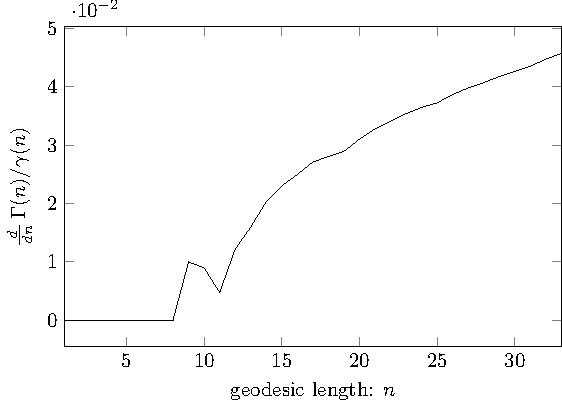
\includegraphics[width=\linewidth]
			{figures/results/normalGrowth/usual/normalGrowthRatioD1}
		\caption{First derivative of $\Gamma(n)/\gamma(n)$}
		\label{fig:normalGrowthRatio:linear:D1}
	\end{subfigure}
	\hfill
	\begin{subfigure}{0.48\linewidth}
		\centering
		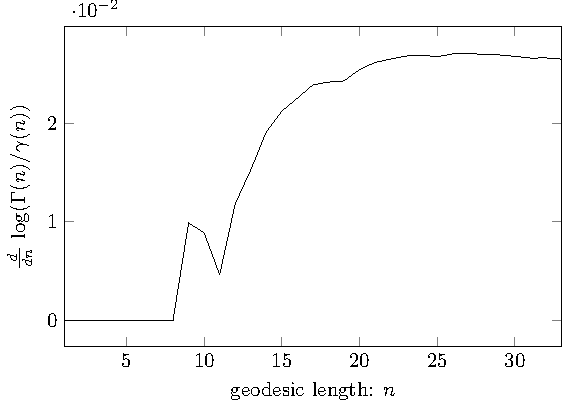
\includegraphics[width=\linewidth]
			{figures/results/normalGrowth/log/normalGrowthRatioLogD1}
		\caption{First derivative of $\log(\Gamma(n)/\gamma(n))$}
		\label{fig:normalGrowthRatio:log:D1}
	\end{subfigure}
	
	\caption{First derivatives of $\Gamma(n)/\gamma(n)$ and $\log(\Gamma(n)/\gamma(n))$}
	\label{fig:normalGrowthRatioD1}
\end{figure}

Further, the second and third derivatives (computed by the central difference) of $\Gamma(n)/\gamma(n)$ are given in \cref{fig:normalGrowthRatioD2D3}.

\begin{figure}[!h]
	\centering
	
	\begin{subfigure}{0.48\linewidth}
		\centering
		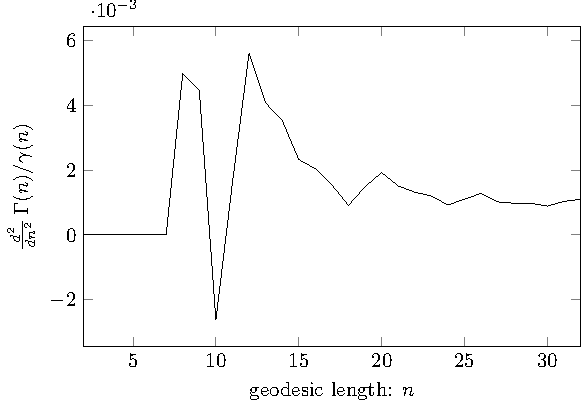
\includegraphics[width=\linewidth]
		{figures/results/normalGrowth/usual/normalGrowthRatioD2}
		\caption{Second derivative of $\Gamma(n)/\gamma(n)$}
		\label{fig:normalGrowthRatio:linear:D2}
	\end{subfigure}
	\hfill
	\begin{subfigure}{0.48\linewidth}
		\centering
		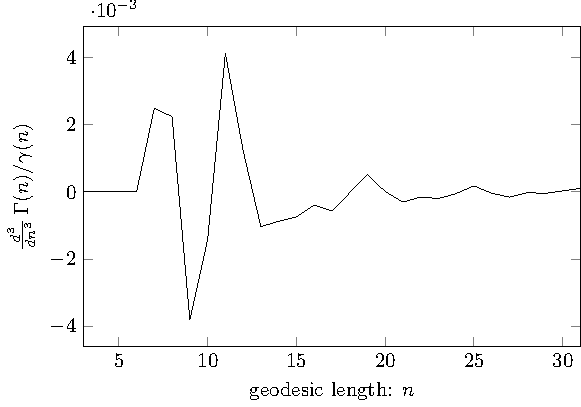
\includegraphics[width=\linewidth]
		{figures/results/normalGrowth/usual/normalGrowthRatioD3}
		\caption{Third derivative of $\Gamma(n)/\gamma(n)$}
		\label{fig:normalGrowthRatio:log:D3}
	\end{subfigure}
	
	\caption{Higher derivatives of $\Gamma(n)/\gamma(n)$}
	\label{fig:normalGrowthRatioD2D3}
\end{figure}

\newpage
\section{Geodesic Equivalence Class Size}

Similar to the previous section, for $\Gamma(n)$ to be subexponential and thus intermediate, it would be sufficient to show that the size of the largest geodesic equivalence class is subexponential with respect to the geodesic length $n$; and further, if such a function is exponential, the so is $\Gamma(n)$.
Thus, the size of the largest equivalence classes is given in \cref{fig:maximumEquivClassSize}.
The corresponding raw data of this section is given in \cref{tab:class-sizes}.

\begin{figure}[!h]
	\centering
	
	\begin{subfigure}{0.48\linewidth}
		\centering
		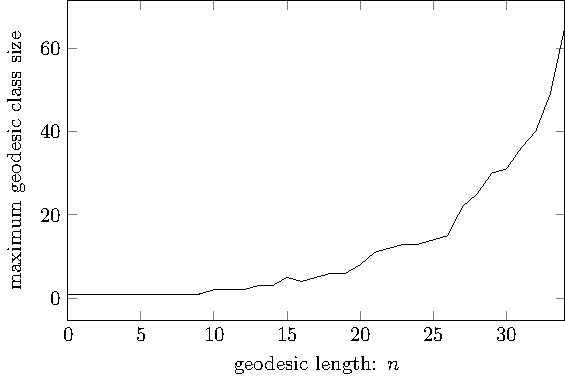
\includegraphics[width=\linewidth]
		{figures/results/maxClassSize/usual/maxClassSize}
		\caption{linear scale}
		\label{fig:maximumEquivClassSize:linear}
	\end{subfigure}
	\hfill
	\begin{subfigure}{0.48\linewidth}
		\centering
		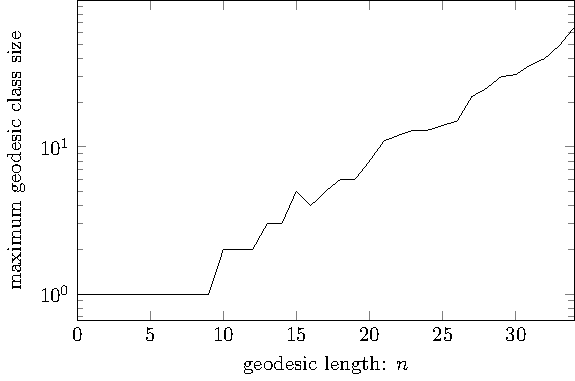
\includegraphics[width=\linewidth]
		{figures/results/maxClassSize/log/maxClassSizeLog}
		\caption{logatithmic scale}
		\label{fig:maximumEquivClassSize:log}
	\end{subfigure}
	
	\caption{The size of the largest equivalence classes}
	\label{fig:maximumEquivClassSize}
\end{figure}

\section{Remarks and Conjecture}

After generating the geodesics described in this section, graphs similar to the one on the front cover of this thesis were generated.
The graph on the cover represents a particular geodesic equivalence class of length 24 geodesics where the first node corresponds the group identity and the last node corresponds the group element represented by the geodesics.
Thus, such graphs can be understood to be sub-graphs of the Cayley graph of the Fabrykowski-Gupta group.

The idea behind generating graphs such as the one on the front cover was to see if any patterns presented themselves.
For example, if any exponential growth sub-families could be seen from such graphs.
The other patterns of this form have not been included in this thesis due to the large number of such graphs; there are $2311$ distinct graphs, of this form, of length 23 geodesics alone.

Considering the figures from the previous two sections, the author arrives at the following conjecture.

\begin{conjecture}
	The function $\Gamma(n)/\gamma(n)$ either grows slower than quadratic or is exponential of a small growth rate; thus either, $\Gamma \preccurlyeq n^2 \gamma$ or $\Gamma(n)$ is exponential of a small growth rate.
\end{conjecture}

